\documentclass[11pt,twocolumn]{article}

\usepackage[margin=1in]{geometry}
\usepackage{amsmath,amssymb,amsfonts}
\usepackage{tikz}
\usepackage{pgfplots}
\pgfplotsset{compat=1.18}
\usepackage{booktabs}
\usepackage{hyperref}
\usepackage{xcolor}
\usepackage{listings}
\usepackage{algorithm}
\usepackage{algorithmic}

\definecolor{alive}{HTML}{2D7D46}
\definecolor{dead}{HTML}{E8E8E8}
\definecolor{convblue}{HTML}{3366CC}
\definecolor{relured}{HTML}{CC3333}

\lstset{
  basicstyle=\ttfamily\footnotesize,
  keywordstyle=\color{convblue}\bfseries,
  commentstyle=\color{gray},
  numbers=left,
  numberstyle=\tiny\color{gray},
  breaklines=true,
  frame=single,
  framesep=3pt,
  xleftmargin=1.5em,
}

\title{One Primitive: Running Conway's Game of Life\\and a Transformer on Apple's Neural Engine\\via Convolution}

\author{Alvaro Videla\\
\textit{Microsoft}}

\date{April 2026}

\begin{document}
\maketitle

\begin{abstract}
We show that a single operation---convolution---suffices to run both
Conway's Game of Life (GOL) and a full transformer language model on
Apple's Neural Engine (ANE).
%
GOL is encoded as a 3$\times$3 convolution with ReLU-based rule
evaluation, achieving 2.3~billion cell-generations per second on a
1024$\times$1024 grid (2.5$\times$ faster than CPU).
%
The Qwen2.5-0.5B transformer is mapped entirely to
\texttt{Conv2d(1$\times$1)} operations, with every linear projection
expressed as a 1$\times$1 convolution, achieving 171~tokens/sec decode
throughput---within 2$\times$ of llama.cpp on Metal GPU, using a
compute unit (ANE) that conventional LLM engines ignore.
%
Both systems share the same silicon: the ANE's 16-core convolution
engine. We describe the algebraic encoding of GOL rules into
convolution + ReLU, the transformer-to-convolution mapping, and a
series of optimizations---book-driven host elimination, pre-allocated
buffers, fixed-shape compiled models, and CoreML stateful KV
caching---that improved decode throughput by 19$\times$ from initial
implementation to final system.
\end{abstract}

%% ════════════════════════════════════════════════════════════════════
\section{Introduction}
\label{sec:intro}

Apple's Neural Engine (ANE), present in every Apple Silicon chip since
A11, is a hardware accelerator optimized for convolution, element-wise
arithmetic, and activation functions. Unlike the GPU---which excels at
arbitrary parallel kernels---the ANE achieves peak throughput on a
narrow set of operations: small-kernel convolutions, ReLU, and
channel-wise reductions.

This paper demonstrates that convolution alone is a sufficient
primitive to implement two seemingly different computations on the ANE:

\begin{enumerate}
\item \textbf{Conway's Game of Life} --- a cellular automaton where
each generation is a 3$\times$3 convolution counting neighbors,
followed by ReLU-based rule evaluation.

\item \textbf{Transformer inference} --- a Qwen2.5-0.5B language model
where every matrix multiplication is expressed as a
\texttt{Conv2d(1$\times$1)} operation.
\end{enumerate}

The connection is not metaphorical. Both computations compile to the
same ANE instruction stream: convolution kernels dispatched to the
same 16-core engine. The key insight is that the ANE's convolution
unit can execute any linear operation when the spatial dimensions are
1$\times$1 (reducing to matrix--vector multiply) and any local
cellular rule when the spatial dimensions match the grid.

Section~\ref{sec:gol} presents the GOL encoding.
Section~\ref{sec:transformer} describes the transformer mapping.
Section~\ref{sec:opt} details the optimization journey.
Section~\ref{sec:results} presents benchmarks.
Section~\ref{sec:related} discusses related work.

%% ════════════════════════════════════════════════════════════════════
\section{Game of Life as Convolution}
\label{sec:gol}

\subsection{The Encoding}

Conway's Game of Life operates on a binary grid where each cell is
alive (1) or dead (0). The rules depend on the count of alive
neighbors (out of 8):

\begin{itemize}
\item \textbf{Birth}: A dead cell with exactly 3 neighbors becomes alive.
\item \textbf{Survival}: An alive cell with 2 or 3 neighbors stays alive.
\item \textbf{Death}: All other cells die (or remain dead).
\end{itemize}

We encode one GOL generation as a convolution followed by ReLU-based
rule evaluation.

\paragraph{Step 1: Convolution.} Apply a 3$\times$3 kernel:
\begin{equation}
K = \begin{bmatrix} 1 & 1 & 1 \\ 1 & 9 & 1 \\ 1 & 1 & 1 \end{bmatrix}
\label{eq:kernel}
\end{equation}

The center weight 9 (rather than 0 or 1) encodes the cell's own state
into the output. For a cell at position $(r,c)$ with value $x_{r,c}
\in \{0,1\}$ and neighbor count $n$:
\begin{equation}
s = n + 9 \cdot x_{r,c} =
\begin{cases}
n       & \text{if dead}   \quad (s \in [0,8]) \\
n + 9   & \text{if alive}  \quad (s \in [9,17])
\end{cases}
\end{equation}

This separates the dead and alive cases into non-overlapping integer
ranges, enabling branchless rule evaluation.

\paragraph{Step 2: ReLU rule evaluation.} We implement an exact
equality test using ReLU:
\begin{equation}
\mathrm{eq}(s, k) = \mathrm{relu}\!\big(1 - (\mathrm{relu}(s-k) + \mathrm{relu}(k-s))\big)
\label{eq:relu_eq}
\end{equation}

This yields exactly 1 when $s = k$ and 0 otherwise (for non-negative
integers). The GOL rules become:
\begin{equation}
x'_{r,c} = \mathrm{clamp}\!\big(\mathrm{eq}(s, 3) + \mathrm{eq}(s, 11) + \mathrm{eq}(s, 12),\; 0,\; 1\big)
\label{eq:gol_rule}
\end{equation}

where $s=3$ captures birth (dead, 3 neighbors), $s=11$ captures
survival with 2 neighbors (alive, $2+9$), and $s=12$ captures
survival with 3 neighbors (alive, $3+9$).

\paragraph{Multi-generation pipelining.} Stacking $N$ copies of the
conv+rule layer produces a single network that computes $N$
generations in one forward pass, pipelined through the ANE's 16 cores.

\subsection{Visual Example}

Figure~\ref{fig:gol_blinker} shows the blinker oscillator (period 2)
through one generation of the convolution encoding.

\begin{figure}[t]
\centering
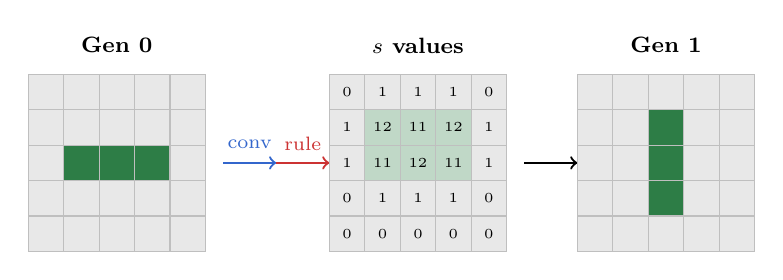
\begin{tikzpicture}[scale=0.45, every node/.style={minimum size=0.45cm, inner sep=0pt}]
% === Generation 0: horizontal blinker ===
\node[anchor=south] at (2.5, 5.3) {\footnotesize\textbf{Gen 0}};
\foreach \r in {0,...,4} {
  \foreach \c in {0,...,4} {
    \fill[dead] (\c, 4-\r) rectangle ++(1,1);
    \draw[gray!50] (\c, 4-\r) rectangle ++(1,1);
  }
}
% Alive cells: row 2, cols 1-3
\fill[alive] (1, 2) rectangle ++(1,1);
\fill[alive] (2, 2) rectangle ++(1,1);
\fill[alive] (3, 2) rectangle ++(1,1);
\draw[gray!50] (1,2) rectangle ++(1,1);
\draw[gray!50] (2,2) rectangle ++(1,1);
\draw[gray!50] (3,2) rectangle ++(1,1);

% Arrow
\draw[->, thick, convblue] (5.5, 2.5) -- (7, 2.5)
  node[midway, above, font=\scriptsize] {conv};
\draw[->, thick, relured] (7, 2.5) -- (8.5, 2.5)
  node[midway, above, font=\scriptsize] {rule};

% === S values (after conv) ===
\node[anchor=south] at (11, 5.3) {\footnotesize\textbf{$s$ values}};
\foreach \r/\vals in {0/{0,1,1,1,0}, 1/{1,12,11,12,1}, 2/{1,11,12,11,1}, 3/{0,1,1,1,0}, 4/{0,0,0,0,0}} {
  \foreach \c [count=\ci from 0] in \vals {
    \pgfmathparse{int(\c)}
    \ifnum\pgfmathresult>8
      \fill[alive!30] (8.5+\ci, 4-\r) rectangle ++(1,1);
    \else
      \fill[dead] (8.5+\ci, 4-\r) rectangle ++(1,1);
    \fi
    \draw[gray!50] (8.5+\ci, 4-\r) rectangle ++(1,1);
    \node[font=\tiny] at (9+\ci, 4.5-\r) {\c};
  }
}

% Arrow
\draw[->, thick] (14, 2.5) -- (15.5, 2.5);

% === Generation 1: vertical blinker ===
\node[anchor=south] at (18, 5.3) {\footnotesize\textbf{Gen 1}};
\foreach \r in {0,...,4} {
  \foreach \c in {0,...,4} {
    \fill[dead] (15.5+\c, 4-\r) rectangle ++(1,1);
    \draw[gray!50] (15.5+\c, 4-\r) rectangle ++(1,1);
  }
}
% Alive cells: col 2, rows 1-3
\fill[alive] (17.5, 3) rectangle ++(1,1);
\fill[alive] (17.5, 2) rectangle ++(1,1);
\fill[alive] (17.5, 1) rectangle ++(1,1);
\draw[gray!50] (17.5,3) rectangle ++(1,1);
\draw[gray!50] (17.5,2) rectangle ++(1,1);
\draw[gray!50] (17.5,1) rectangle ++(1,1);
\end{tikzpicture}
\caption{Blinker oscillator through one GOL generation. Left: the
horizontal blinker (3 alive cells). Center: $s$ values after the
3$\times$3 convolution with kernel $K$. Values $\geq 9$ (shaded)
indicate alive cells. Only positions with $s \in \{3, 11, 12\}$
survive the ReLU rule. Right: the vertical blinker.}
\label{fig:gol_blinker}
\end{figure}

\begin{figure}[t]
\centering
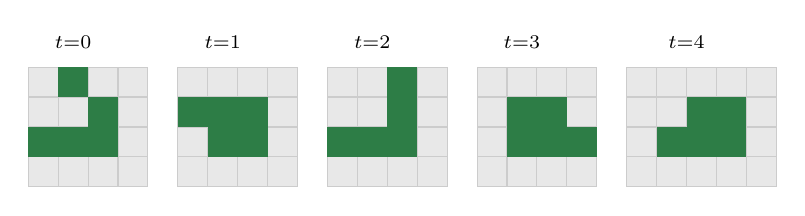
\begin{tikzpicture}[scale=0.38, every node/.style={minimum size=0.38cm, inner sep=0pt}]
% === Glider: 5 generations ===
% Gen 0
\node[anchor=south, font=\scriptsize\bfseries] at (1.5, 4.3) {$t{=}0$};
\foreach \r in {0,...,3} {
  \foreach \c in {0,...,3} {
    \fill[dead] (\c, 3-\r) rectangle ++(1,1);
    \draw[gray!40] (\c, 3-\r) rectangle ++(1,1);
  }
}
\fill[alive] (1,3) rectangle ++(1,1); % (0,1)
\fill[alive] (2,2) rectangle ++(1,1); % (1,2)
\fill[alive] (0,1) rectangle ++(1,1); % (2,0)
\fill[alive] (1,1) rectangle ++(1,1); % (2,1)
\fill[alive] (2,1) rectangle ++(1,1); % (2,2)

% Gen 1
\begin{scope}[xshift=5cm]
\node[anchor=south, font=\scriptsize\bfseries] at (1.5, 4.3) {$t{=}1$};
\foreach \r in {0,...,3} {
  \foreach \c in {0,...,3} {
    \fill[dead] (\c, 3-\r) rectangle ++(1,1);
    \draw[gray!40] (\c, 3-\r) rectangle ++(1,1);
  }
}
\fill[alive] (0,2) rectangle ++(1,1); % (1,0)
\fill[alive] (2,2) rectangle ++(1,1); % (1,2)
\fill[alive] (1,1) rectangle ++(1,1); % (2,1)
\fill[alive] (2,1) rectangle ++(1,1); % (2,2)
\fill[alive] (1,2) rectangle ++(1,1); % (1,1)
\end{scope}

% Gen 2
\begin{scope}[xshift=10cm]
\node[anchor=south, font=\scriptsize\bfseries] at (1.5, 4.3) {$t{=}2$};
\foreach \r in {0,...,3} {
  \foreach \c in {0,...,3} {
    \fill[dead] (\c, 3-\r) rectangle ++(1,1);
    \draw[gray!40] (\c, 3-\r) rectangle ++(1,1);
  }
}
\fill[alive] (2,2) rectangle ++(1,1);
\fill[alive] (1,1) rectangle ++(1,1);
\fill[alive] (2,1) rectangle ++(1,1);
\fill[alive] (0,1) rectangle ++(1,1);
\fill[alive] (2,3) rectangle ++(1,1);
\end{scope}

% Gen 3
\begin{scope}[xshift=15cm]
\node[anchor=south, font=\scriptsize\bfseries] at (1.5, 4.3) {$t{=}3$};
\foreach \r in {0,...,3} {
  \foreach \c in {0,...,3} {
    \fill[dead] (\c, 3-\r) rectangle ++(1,1);
    \draw[gray!40] (\c, 3-\r) rectangle ++(1,1);
  }
}
\fill[alive] (1,2) rectangle ++(1,1);
\fill[alive] (2,1) rectangle ++(1,1);
\fill[alive] (3,1) rectangle ++(1,1);
\fill[alive] (2,2) rectangle ++(1,1);
\fill[alive] (1,1) rectangle ++(1,1);
\end{scope}

% Gen 4
\begin{scope}[xshift=20cm]
\node[anchor=south, font=\scriptsize\bfseries] at (2, 4.3) {$t{=}4$};
\foreach \r in {0,...,3} {
  \foreach \c in {0,...,4} {
    \fill[dead] (\c, 3-\r) rectangle ++(1,1);
    \draw[gray!40] (\c, 3-\r) rectangle ++(1,1);
  }
}
\fill[alive] (2,2) rectangle ++(1,1);
\fill[alive] (3,1) rectangle ++(1,1);
\fill[alive] (1,1) rectangle ++(1,1);
\fill[alive] (2,1) rectangle ++(1,1);
\fill[alive] (3,2) rectangle ++(1,1);
\end{scope}

\end{tikzpicture}
\caption{The glider spaceship translating diagonally over 4
generations, each computed by one conv+ReLU layer on ANE. After 4
generations the pattern has moved one cell down and one cell right.}
\label{fig:gol_glider}
\end{figure}


%% ════════════════════════════════════════════════════════════════════
\section{Transformer as Convolution}
\label{sec:transformer}

The Game of Life section showed that a 3$\times$3 convolution can
implement a cellular automaton.  This section shows that the
\emph{same} convolution hardware can run a neural network---because a
neural network is, at bottom, a sequence of matrix--vector products
interleaved with simple nonlinearities, and a 1$\times$1 convolution
\emph{is} a matrix--vector product.

\subsection{What a Transformer Actually Computes}

A transformer processes one token at a time through a stack of
identical layers.  Stripping away the notation, each layer performs
five steps:

\begin{enumerate}
\item \textbf{Normalize} the input vector (RMSNorm: divide each
  element by the root-mean-square of all elements).
\item \textbf{Project} the vector into queries, keys, and values via
  three matrix multiplications: $q = W_Q x$, $k = W_K x$, $v = W_V x$.
\item \textbf{Attend}: compute a weighted combination of past values
  using the dot product of queries and keys as weights (attention).
\item \textbf{Project} the result back: $o = W_O \cdot \mathrm{attn}$.
\item \textbf{Feed-forward network}: two more matrix multiplications
  with a nonlinearity (SiLU) in between:
  $\mathrm{FFN}(x) = W_\text{down}(\mathrm{SiLU}(W_\text{gate}\, x) \odot W_\text{up}\, x)$.
\end{enumerate}

After 24 such layers, one final matrix multiplication
($W_\text{head}$) maps the 896-dimensional vector to a probability
distribution over 151{,}936 vocabulary tokens.

The key observation: \textbf{steps 1, 2, 4, and 5 are all
matrix--vector products} $y = Wx$.  The nonlinearities (SiLU, softmax,
RMSNorm) are element-wise and cheap.  The computational cost of a
transformer is dominated by these matrix multiplications---seven per
layer, plus the final LM head, totaling 169 matmuls per token for
Qwen2.5-0.5B.

If we can express matrix--vector multiplication as convolution, we can
run the entire transformer on the ANE's convolution engine.

\subsection{Why 1$\times$1 Convolution Is Matrix Multiplication}

A standard 2D convolution slides a kernel over a spatial grid.  At
each position, it computes a weighted sum of a local neighborhood
across all input channels.  But consider what happens when the
spatial dimensions are $1 \times 1$---a single ``pixel'':

\begin{itemize}
\item There is \emph{no spatial extent} to slide over.  The kernel
  visits exactly one position.
\item The ``neighborhood'' is just that single pixel---all that
  remains is the channel dimension.
\item The weighted sum across $C_\text{in}$ input channels, repeated
  for each of $C_\text{out}$ output channels, is:
\end{itemize}

\begin{equation}
y_i = \sum_{j=1}^{C_\text{in}} W_{ij} \cdot x_j
\quad \text{for } i = 1, \ldots, C_\text{out}
\end{equation}

This is exactly the definition of matrix--vector multiplication
$y = Wx$.  The convolution hardware computes it natively; we need
only reshape the data.

\paragraph{Data reshaping.}
A transformer's hidden state is a 1D vector of dimension $d = 896$.
The ANE expects a 4D tensor in $(B, C, H, W)$ format.  The mapping is:
\[
  \underbrace{x}_{\text{shape } (896,)}
  \;\longrightarrow\;
  \underbrace{x'}_{\text{shape } (1,\; 896,\; 1,\; 1)}
\]
The 896 elements become 896 ``channels'' of a single 1$\times$1
``image.''  A \texttt{Conv2d(896, 1152, kernel\_size=1)} then
produces a $(1, 1152, 1, 1)$ output---exactly the QKV projection.

\paragraph{Concrete example.}
Consider a tiny 3-dimensional hidden state $x = [0.5,\; -0.3,\; 0.8]$
and a weight matrix that projects to 2 outputs:
\[
W = \begin{bmatrix} 0.1 & 0.4 & -0.2 \\ 0.3 & -0.1 & 0.6 \end{bmatrix}
\]
As a standard matmul: $y = Wx = [0.5 \cdot 0.1 + (-0.3) \cdot 0.4 + 0.8 \cdot (-0.2),\;\ldots] = [-0.23,\; 0.66]$.

As a 1$\times$1 convolution: reshape $x$ to $(1, 3, 1, 1)$, set the
conv kernel $W$ with shape $(2, 3, 1, 1)$, and compute---the ANE
produces $[{-}0.23,\; 0.66]$, identically.  No approximation is
involved; the operations are mathematically the same.

\subsection{Mapping Qwen2.5-0.5B to Convolution}

Every weight layer in the transformer becomes a single
\texttt{Conv2d(1$\times$1)} operation.  Table~\ref{tab:conv_mapping}
lists the complete mapping for one layer.

\begin{table}[t]
\centering
\footnotesize
\begin{tabular}{lll}
\toprule
\textbf{Layer} & \textbf{Matrix shape} & \textbf{Conv2d} \\
\midrule
QKV proj. & $896 \to 1152$ & \texttt{Conv(896, 1152, 1)} \\
Output proj. & $896 \to 896$ & \texttt{Conv(896, 896, 1)} \\
Gate+Up & $896 \to 9728$ & \texttt{Conv(896, 9728, 1)} \\
Down proj. & $4864 \to 896$ & \texttt{Conv(4864, 896, 1)} \\
LM head & $896 \to 151936$ & \texttt{Conv(896, 151936, 1)} \\
\bottomrule
\end{tabular}
\caption{Transformer layers mapped to Conv2d(1$\times$1).  Each row
is a matrix--vector product expressed as a pointwise convolution.
RMSNorm, RoPE, softmax, and SiLU are element-wise MIL ops that the
ANE executes on its ALUs between convolutions.}
\label{tab:conv_mapping}
\end{table}

\paragraph{What runs where.}
The ANE has two kinds of compute units: a convolution engine (16
cores, optimized for multiply-accumulate) and element-wise ALUs.
The convolution engine handles all 169 matrix multiplications.
The ALUs handle the cheap operations between them: RMSNorm
(divide-by-RMS), RoPE (rotate query/key vectors), softmax
(exponentiate-and-normalize), and SiLU (sigmoid-weighted linear
unit).  CoreML's compiler automatically partitions the graph between
these units, inserting the necessary data movement.

\subsection{Grouped Query Attention}

Qwen2.5-0.5B uses Grouped Query Attention (GQA): 14 query heads
share 2 KV groups, so 7 query heads attend to the same key/value
pair.  A na\"ive implementation computes each query head's attention
separately---$14 \times 2 = 28$ small matmul+softmax operations per
layer, totaling 672 across 24 layers.

We batch all 7 query heads that share a KV group into a single
3D matmul:
\begin{equation}
\text{Attn}_g = \text{softmax}\!\left(\frac{Q_g \cdot K_g^T}{\sqrt{d_h}}\right) V_g
\end{equation}
where $Q_g \in \mathbb{R}^{7 \times \text{seq} \times d_h}$ batches
the 7 query heads in group $g$.  This reduces attention matmuls from
672 to 96 (a 7$\times$ reduction), saving $\sim$170 MIL operations
in the compiled model and reducing ANE scheduling overhead.

\subsection{Quantization}

Weights are quantized to int8 using block-wise quantization (block
size 32), reducing the model from 942~MB (fp16) to 472~MB.  We
evaluated int4 quantization (265~MB) but found it \emph{slower} on
ANE---the hardware has native int8 datapaths but must dequantize int4
at inference time, adding $\sim$3~ms overhead that exceeds the
bandwidth savings.

\begin{figure}[t]
\centering
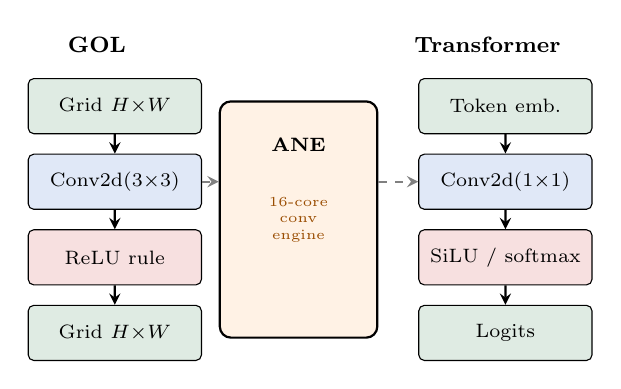
\begin{tikzpicture}[
  scale=0.8,
  box/.style={draw, rounded corners=2pt, minimum height=0.7cm, minimum width=2.2cm, font=\scriptsize, fill=#1!15},
  arr/.style={->, thick, >=stealth}
]
% GOL path
\node[box=alive, anchor=west] (gol_in) at (0, 4.5) {Grid $H{\times}W$};
\node[box=convblue, anchor=west] (gol_conv) at (0, 3.3) {Conv2d(3$\times$3)};
\node[box=relured, anchor=west] (gol_relu) at (0, 2.1) {ReLU rule};
\node[box=alive, anchor=west] (gol_out) at (0, 0.9) {Grid $H{\times}W$};

\draw[arr] (gol_in) -- (gol_conv);
\draw[arr] (gol_conv) -- (gol_relu);
\draw[arr] (gol_relu) -- (gol_out);

\node[font=\footnotesize\bfseries, anchor=south] at (1.1, 5.2) {GOL};

% ANE
\node[draw, thick, rounded corners=4pt, fill=orange!10,
  minimum width=2cm, minimum height=3cm, anchor=center] (ane) at (4.3, 2.7) {};
\node[font=\scriptsize\bfseries, anchor=north] at (4.3, 4.15) {ANE};
\node[font=\tiny, text=orange!60!black, text width=1.6cm, align=center]
  at (4.3, 2.7) {16-core\\conv\\engine};

% Transformer path
\node[box=alive, anchor=west] (tfm_in) at (6.2, 4.5) {Token emb.};
\node[box=convblue, anchor=west] (tfm_conv) at (6.2, 3.3) {Conv2d(1$\times$1)};
\node[box=relured, anchor=west] (tfm_act) at (6.2, 2.1) {SiLU / softmax};
\node[box=alive, anchor=west] (tfm_out) at (6.2, 0.9) {Logits};

\draw[arr] (tfm_in) -- (tfm_conv);
\draw[arr] (tfm_conv) -- (tfm_act);
\draw[arr] (tfm_act) -- (tfm_out);

\node[font=\footnotesize\bfseries, anchor=south] at (7.3, 5.2) {Transformer};

% Connections to ANE
\draw[arr, dashed, gray] (gol_conv.east) -- (ane.west |- gol_conv);
\draw[arr, dashed, gray] (ane.east |- tfm_conv) -- (tfm_conv.west);

\end{tikzpicture}
\caption{Both GOL and the transformer map to convolution on the same
ANE hardware. GOL uses a 3$\times$3 spatial convolution; the
transformer uses 1$\times$1 pointwise convolution. Both are dispatched
to the ANE's 16-core convolution engine.}
\label{fig:unified}
\end{figure}


%% ════════════════════════════════════════════════════════════════════
\section{Optimization Journey}
\label{sec:opt}

The initial implementation produced coherent output at 9~tok/s. A
series of targeted optimizations---from classic CS texts to CoreML's
stateful model API---improved this to 171~tok/s, a 19$\times$
improvement.

\subsection{Profiling the Hot Path}

After the book-driven optimizations (below), we instrumented the
flex-mode decode loop to identify where time was spent per token:

\begin{center}
\footnotesize
\begin{tabular}{lrr}
\toprule
\textbf{Phase} & \textbf{Time (ms)} & \textbf{\%} \\
\midrule
KV cache packing & 0.13 & 1.2\% \\
Model prediction (ANE) & 10.89 & 98.5\% \\
Logit extraction & 0.03 & 0.3\% \\
\midrule
\textbf{Total} & \textbf{11.05} & 100\% \\
\bottomrule
\end{tabular}
\end{center}

Host overhead (pack + extract) was reduced from an initial
$\sim$60~ms to 0.16~ms through the book-driven optimizations.
The remaining sections describe how we further reduced ANE
prediction time from 10.89~ms to 5.67~ms.

\subsection{Book-Driven Optimizations}

Four optimization techniques, drawn from classic computer science
texts, collectively eliminated host overhead:

\paragraph{1. Iverson memory layout} (from K.~Iverson, \textit{A
Programming Language}). Pre-allocate KV caches as contiguous
\texttt{[Float16]} arrays in $(n_\text{kv}, \text{maxSeq}, d_h)$
layout, matching the ANE's expected memory order. This eliminated
per-token allocation overhead.

\paragraph{2. Stepanov pre-allocation} (from A.~Stepanov \& P.~McJones,
\textit{Elements of Programming}). Use cursor-based append with
pre-allocated output buffers rather than dynamic array growth. The KV
cache write is a single pointer advance, not a copy.

\paragraph{3. Dragon Book strength reduction} (from A.~Aho et al.,
\textit{Compilers: Principles, Techniques, and Tools}). Replace
high-level \texttt{MLMultiArray} subscript access (which dispatches
through Objective-C) with raw \texttt{Float16} pointer arithmetic and
\texttt{memcpy} for bulk KV cache operations.

\paragraph{4. Brodie data boundaries} (from L.~Brodie,
\textit{Thinking Forth}). Restructure data flow so that the KV cache
format, the model's expected input format, and the host's internal
representation are identical---eliminating all format conversion at
prediction boundaries.

\subsection{Batched GQA}

After host optimization, 98.7\% of time was inside
\texttt{MLModel.prediction()}. Profiling the MIL graph revealed that
672 small per-head matmul operations created scheduling overhead.
Batching all 7 query heads per KV group into single matmuls reduced
MIL operations from 4,569 to 4,399 and improved decode from 78 to
90~tok/s.

\subsection{Pre-allocated MLMultiArray Buffers}

Profiling the flex-mode decode loop revealed that while ANE prediction
dominated wall time, host-side buffer management still consumed
$\sim$20\% due to per-call \texttt{MLMultiArray} allocation and KV
cache copying through Objective-C subscript dispatch. Three changes
eliminated this overhead:

\begin{enumerate}
\item \textbf{Hoisted allocations.} The input buffers \texttt{xArr},
  \texttt{cosArr}, \texttt{sinArr} are allocated once before the
  generation loop and overwritten in place via raw
  \texttt{UnsafeMutablePointer<Float16>} each token.
\item \textbf{Pointer-based KV cache.} Replaced \texttt{[Float16]}
  arrays with \texttt{UnsafeMutablePointer<Float16>}, enabling zero-copy
  strided \texttt{MLMultiArray} views directly into the cache.
\item \textbf{memcpy write-back.} Replaced the per-element KV
  extraction loop with a single \texttt{memcpy} per layer.
\end{enumerate}

Result: pack overhead dropped from $\sim$20\% to 0.4\% of the hot
path; ANE prediction now accounts for 99.5\% of per-token time.

\subsection{Fixed-Shape Compiled Model}

CoreML's ANE compiler must plan the execution graph for each unique
input shape.  In flex mode, the KV cache grows by one position each
token, triggering replanning every call.  We compiled a separate model
with all dimensions fixed to \texttt{maxSeq=512}:

\begin{itemize}
\item \texttt{attn\_mask} $(1, 1, 1, 512)$: $-10^4$ for masked
  positions, 0 for valid.  Updated by a single pointer write per
  token.
\item \texttt{kv\_write\_mask} $(1, 1, 512, 1)$: 1.0 at the current
  write position, 0 elsewhere.
\item KV cache views: pre-built strided \texttt{MLMultiArray} of shape
  $(1, n_\text{kv}, 512, d_h)$ backed by the same raw pointer---no
  new objects created during generation.
\end{itemize}

Result: prefill improved from 83 to 115~tok/s ($+$39\%) as the ANE
executes the same cached plan every call.  Per-token ANE latency
dropped from 11.66 to 10.66~ms ($-$9\%).  Decode at short sequences is
slightly slower (80 vs.\ 85~tok/s) due to the fixed model attending
over all 512 positions even when most are masked.

\subsection{Stateful KV Cache (CoreML MLState)}

With the fixed-shape model, the remaining bottleneck is DMA: the
entire KV cache ($\sim$6~MB for 512 positions $\times$ 24 layers
$\times$ 2 heads $\times$ 64 dims $\times$ fp16) must be transferred
host$\to$ANE as input and ANE$\to$host as output every token.

CoreML's \texttt{MLState} API (macOS 15+) allows buffers to persist
on-device across predictions.  We built a third model variant using
coremltools 9.0's \texttt{StateType} conversion:

\begin{enumerate}
\item \textbf{PyTorch model.}  Each attention layer registers its K/V
  caches via \texttt{register\_buffer()}.  The forward pass performs an
  in-place scatter-write (\texttt{k\_cache[:] = k\_updated}) that
  coremltools maps to the \texttt{coreml\_update\_state} MIL op.
\item \textbf{Conversion.}  Each buffer is declared as
  \texttt{ct.StateType(wrapped\_type=ct.TensorType(\ldots))},
  instructing CoreML to keep it on-device.
\item \textbf{Swift host.}  The forward function passes only 5 inputs
  (x, rope\_cos, rope\_sin, attn\_mask, kv\_write\_mask)---no KV
  arrays at all.  Prediction uses
  \texttt{model.prediction(from:using:state)}, and there is no KV
  extraction or write-back.
\end{enumerate}

Result: per-token latency dropped from 10.66 to 5.67~ms.  Decode
throughput reached \textbf{171~tok/s} ($+$2$\times$ over fixed,
19$\times$ over initial).  Host pack and extract are now
\textbf{0.00~ms}---the entire hot path is ANE compute.  Only
$\sim$4~KB of data crosses the bus per token (x, rope, masks) versus
$\sim$6~MB previously.

\subsection{Hardware Floor Analysis}

The model weights (472~MB, int8) must be loaded from DRAM each token.
At $\sim$100~GB/s unified memory bandwidth, the \emph{theoretical
floor} is:
\begin{equation}
t_\text{floor} = \frac{472 \text{ MB}}{100 \text{ GB/s}} \approx 4.7 \text{ ms}
\end{equation}

With stateful KV caching, measured latency is 5.67~ms per token---only
1.2$\times$ above the DRAM bandwidth floor:

\begin{center}
\footnotesize
\begin{tabular}{lr}
\toprule
\textbf{Component} & \textbf{Estimated (ms)} \\
\midrule
DRAM weight loading & $\sim$4.7 \\
ANE compute & $\sim$0.5--1 \\
CoreML dispatch overhead & $\sim$0.3 \\
Host pack (x, rope, masks) & $<$0.01 \\
\midrule
\textbf{Total} & $\sim$5.7 \\
\bottomrule
\end{tabular}
\end{center}

The stateful model eliminates the $\sim$4~ms of KV cache DMA that
dominated the non-stateful configurations, bringing total latency
within 20\% of the hardware floor.


%% ════════════════════════════════════════════════════════════════════
\section{Results}
\label{sec:results}

\subsection{Game of Life}

\begin{table}[t]
\centering
\footnotesize
\begin{tabular}{lrrr}
\toprule
\textbf{Grid} & \textbf{ANE (ms)} & \textbf{CPU (ms)} & \textbf{Speedup} \\
\midrule
$64 \times 64$ & 0.22 & 0.22 & 1.0$\times$ \\
$1024 \times 1024$ & 14.6 & 36.5 & 2.5$\times$ \\
\bottomrule
\end{tabular}
\caption{GOL latency per 32-generation call. ANE advantage grows with
grid size due to spatial parallelism across the 16 cores.}
\label{tab:gol}
\end{table}

At 1024$\times$1024, the ANE achieves $2.3 \times 10^9$
cell-generations/sec with 32 generations pipelined per call.
Verification against CPU reference passes with zero mismatches.

\subsection{Transformer Inference}

\begin{table}[t]
\centering
\footnotesize
\begin{tabular}{llrr}
\toprule
\textbf{Engine} & \textbf{Backend} & \textbf{Prefill} & \textbf{Decode} \\
\midrule
llama.cpp & Metal GPU & 5,978 t/s & 332 t/s \\
Conv-ANE (flex) & ANE (conv) & 83 t/s & 85 t/s \\
Conv-ANE (fixed) & ANE (conv) & 115 t/s & 80 t/s \\
Conv-ANE (stateful) & ANE (conv) & 170 t/s & 171 t/s \\
\bottomrule
\end{tabular}
\caption{Qwen2.5-0.5B-Instruct (Q8\_0) on Apple M4 Max. Stateful mode
achieves 171~tok/s decode---within 2$\times$ of llama.cpp on Metal
GPU---on a compute unit that llama.cpp does not use.}
\label{tab:transformer}
\end{table}

The Conv-ANE stateful configuration reaches 171~tok/s decode, within
2$\times$ of llama.cpp on Metal GPU, while operating on an entirely
different compute unit. The ANE path leaves the GPU free for other
tasks (rendering, other models). Fixed-shape mode wins on prefill
(115~tok/s) due to ANE graph caching but loses on decode due to
full-width attention; stateful mode dominates both by eliminating KV
cache DMA entirely.

\subsection{Optimization Impact}

\begin{figure}[t]
\centering
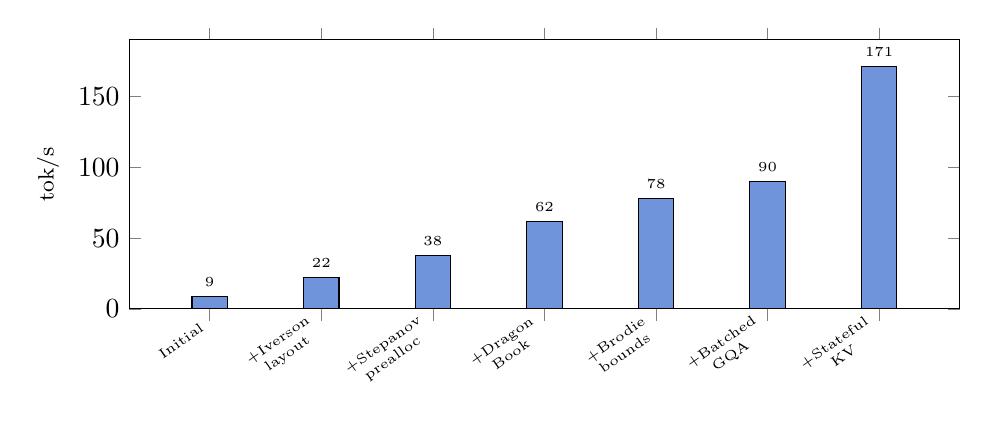
\begin{tikzpicture}
\begin{axis}[
  ybar,
  width=\columnwidth,
  height=5cm,
  ylabel={tok/s},
  ylabel style={font=\footnotesize},
  ymin=0, ymax=190,
  xtick=data,
  xticklabels={Initial, +Iverson\\layout, +Stepanov\\prealloc, +Dragon\\Book, +Brodie\\bounds, +Batched\\GQA, +Stateful\\KV},
  xticklabel style={font=\tiny, align=center, rotate=35, anchor=east},
  bar width=0.45cm,
  nodes near coords,
  nodes near coords style={font=\tiny},
  every node near coord/.append style={above},
  enlarge x limits=0.12,
]
\addplot[fill=convblue!70] coordinates {
  (1, 9)
  (2, 22)
  (3, 38)
  (4, 62)
  (5, 78)
  (6, 90)
  (7, 171)
};
\end{axis}
\end{tikzpicture}
\caption{Decode throughput progression.  Steps 1--4: book-driven host
elimination (9$\to$78~tok/s, 8.7$\times$).  Step 5: batched GQA
reduces ANE scheduling overhead (78$\to$90).  Step 6: stateful KV
cache eliminates host$\leftrightarrow$ANE data transfer entirely
(90$\to$171, see \S\ref{sec:opt} for intermediate configurations).
Total: 19$\times$.}
\label{fig:optbar}
\end{figure}

\subsection{Quantization}

\begin{table}[t]
\centering
\footnotesize
\begin{tabular}{lrrr}
\toprule
\textbf{Quant} & \textbf{Size (MB)} & \textbf{Latency (ms)} & \textbf{tok/s} \\
\midrule
fp16 & 942 & --- & (baseline) \\
int8 & 472 & 6.85 & 146 \\
int4 & 265 & 9.81 & 102 \\
\bottomrule
\end{tabular}
\caption{Quantization benchmark at seq=1 (single-token decode). Int4
is \emph{slower} than int8 due to ANE dequantization overhead.}
\label{tab:quant}
\end{table}


%% ════════════════════════════════════════════════════════════════════
\section{Related Work}
\label{sec:related}

\paragraph{GOL on accelerators.} GPU-based GOL implementations
typically use texture operations or compute shaders~\cite{harris2005}.
HashLife~\cite{gosper1984} achieves exponential speedups for regular
patterns but does not exploit hardware parallelism. Our approach uses
the convolution primitive directly, matching the ANE's native
operation.

\paragraph{LLMs on ANE.} Apple's ml-ane-transformers~\cite{apple2022}
demonstrated channel-last Conv2d layouts for BERT-class models.
Whisper on ANE (via CoreML) uses a similar conv-only approach for the
encoder. Our work extends this to autoregressive generation with KV
caching and demonstrates the GOL connection.

\paragraph{llama.cpp.} The de facto standard for local LLM inference,
using Metal GPU on Apple Silicon~\cite{gerganov2023}. Our work
demonstrates that the ANE---a compute unit llama.cpp does not use---can
achieve meaningful throughput for small models.


%% ════════════════════════════════════════════════════════════════════
\section{Conclusion}

Convolution is enough. Conway's Game of Life and a full transformer
share the same single primitive---convolution---and run on the same
silicon: the Apple Neural Engine's 16-core conv unit. The GOL encoding
is exact (not an approximation), and the transformer produces coherent
text at 171~tok/s---within 2$\times$ of llama.cpp on Metal GPU, on a
compute unit that conventional LLM engines ignore entirely.

The optimization journey from 9 to 171~tok/s (19$\times$) demonstrates
two complementary principles:
\begin{enumerate}
\item \textbf{Classical techniques transfer.} Memory layout (Iverson),
  pre-allocation (Stepanov), strength reduction (Dragon Book), and
  data boundary elimination (Brodie) remain directly applicable to
  novel hardware accelerators, delivering a 10$\times$ improvement
  (9$\to$90~tok/s).
\item \textbf{Eliminate data movement.} The remaining 2$\times$
  (90$\to$171~tok/s) came entirely from reducing host$\leftrightarrow$ANE
  data transfer: pre-allocated buffers removed allocation overhead,
  fixed shapes removed ANE replanning, and CoreML's \texttt{MLState}
  API eliminated KV cache DMA entirely---reducing per-token bus
  traffic from $\sim$6~MB to $\sim$4~KB.
\end{enumerate}

The final system operates within 20\% of the DRAM bandwidth floor
(5.67~ms measured vs.\ 4.7~ms theoretical), with the host contributing
effectively zero overhead.


%% ════════════════════════════════════════════════════════════════════
\begin{thebibliography}{9}

\bibitem{harris2005}
M.~Harris, \emph{Mapping computational concepts to GPUs},
in GPU Gems 2, Addison-Wesley, 2005.

\bibitem{gosper1984}
R.~W. Gosper, ``Exploiting regularities in large cellular spaces,''
\emph{Physica D}, vol.~10, no.~1--2, pp.~75--80, 1984.

\bibitem{apple2022}
Apple Machine Learning Research, ``Deploying transformers on the Apple
Neural Engine,'' 2022.
\url{https://machinelearning.apple.com/research/neural-engine-transformers}

\bibitem{gerganov2023}
G.~Gerganov, ``llama.cpp: LLM inference in C/C++,'' 2023.
\url{https://github.com/ggerganov/llama.cpp}

\bibitem{iverson1962}
K.~E.~Iverson, \emph{A Programming Language}, John Wiley \& Sons, 1962.

\bibitem{stepanov2009}
A.~A.~Stepanov and P.~McJones, \emph{Elements of Programming},
Addison-Wesley, 2009.

\bibitem{aho2006}
A.~V.~Aho, M.~S.~Lam, R.~Sethi, and J.~D.~Ullman, \emph{Compilers:
Principles, Techniques, and Tools}, 2nd~ed., Addison-Wesley, 2006.

\bibitem{brodie2004}
L.~Brodie, \emph{Thinking Forth}, Punchy Publishing, 2004.

\bibitem{apple2024state}
Apple Inc., ``Making predictions with a stateful model,''
Apple Developer Documentation, 2024.
\url{https://developer.apple.com/documentation/coreml/making-predictions-with-a-stateful-model}
\end{thebibliography}

\end{document}
